\section{Results}

\begin{frame}{Results}{Three Cluster Case}
    Using the K-Nearest Neighbors Graph with Uniform Weights
    \begin{figure}[h!]
        \begin{subfigure}[b]{0.45\textwidth}
            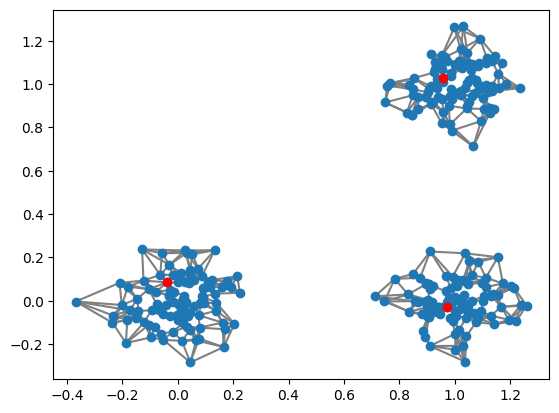
\includegraphics[width=\textwidth]{tc_knn.png}
        \end{subfigure}
        \begin{subfigure}[b]{0.45\textwidth}
            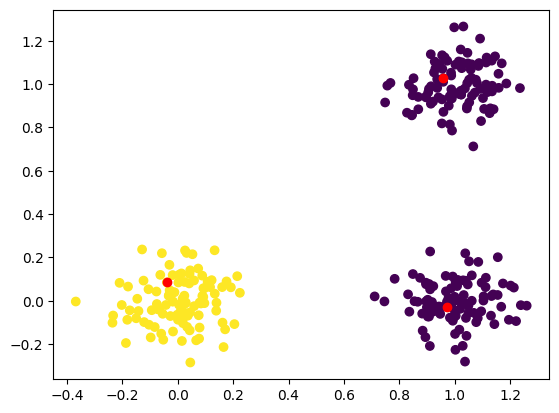
\includegraphics[width=\textwidth]{tc_result.png}
        \end{subfigure}
    \end{figure}
    \begin{center}
        \begin{tabular}{|c|c|}
            \hline
            Loss Function & Classification Accuracy (over 50 trials) \\
            \hline
            Probit & 100.0\% \\
            Regression & 100.0\% \\
            \hline
        \end{tabular}
    \end{center}
\end{frame}

\begin{frame}{Results}{Three Cluster Case}
    Using the Proximity Graph with RBF Weights
    \begin{figure}[h!]
        \begin{subfigure}[b]{0.45\textwidth}
            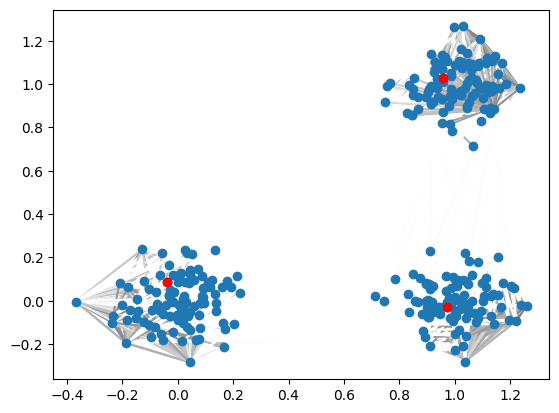
\includegraphics[width=\textwidth]{tc_prox.png}
        \end{subfigure}
        \begin{subfigure}[b]{0.45\textwidth}
            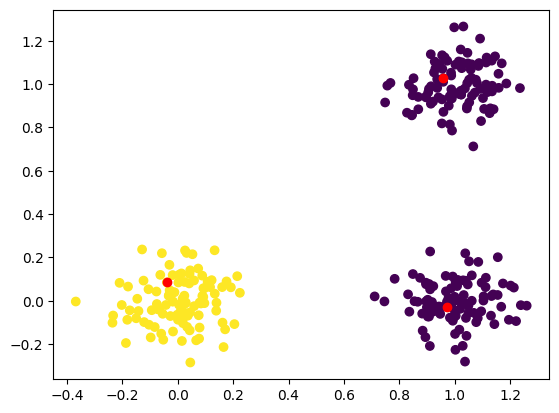
\includegraphics[width=\textwidth]{tc_result.png}
        \end{subfigure}
    \end{figure}
    \begin{center}
        \begin{tabular}{|c|c|}
            \hline
            Loss Function & Classification Accuracy (over 50 trials) \\
            \hline
            Probit & 100.0\% \\
            Regression & 100.0\% \\
            \hline
        \end{tabular}
    \end{center}
\end{frame}

\begin{frame}{Results}{Spiral Case}
    Using the K-Nearest Neighbors Graph with RBF Weights
    \begin{figure}[h!]
        \begin{subfigure}[b]{0.45\textwidth}
            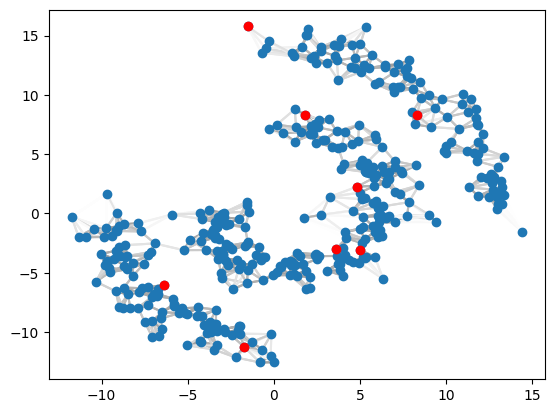
\includegraphics[width=\textwidth]{spiral_knn.png}
        \end{subfigure}
        \begin{subfigure}[b]{0.45\textwidth}
            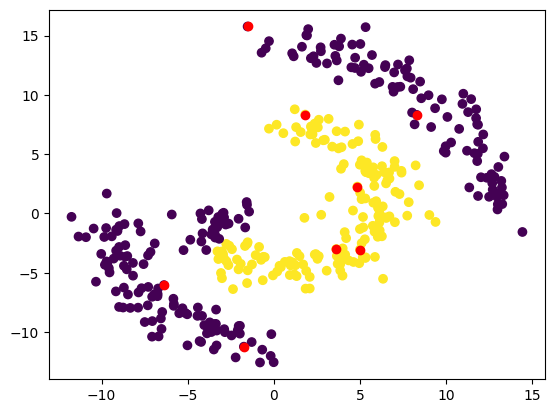
\includegraphics[width=\textwidth]{spiral_knn_r.png}
        \end{subfigure}
    \end{figure}
    \begin{center}
        \begin{tabular}{|c|c|}
            \hline
            Loss Function & Classification Accuracy (over 50 trials) \\
            \hline
            Probit & 96.3\% \\
            Regression & 95.8\% \\
            \hline
        \end{tabular}
    \end{center}
\end{frame}

\begin{frame}{Results}{Spiral Case}
    Using the Proximity Graph with RBF Weights
    \begin{figure}[h!]
        \begin{subfigure}[b]{0.45\textwidth}
            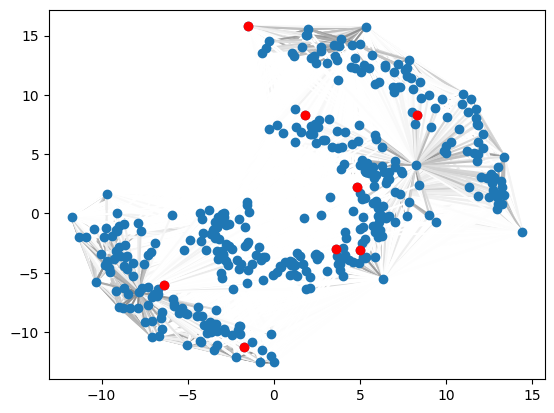
\includegraphics[width=\textwidth]{spiral_prox.png}
        \end{subfigure}
        \begin{subfigure}[b]{0.45\textwidth}
            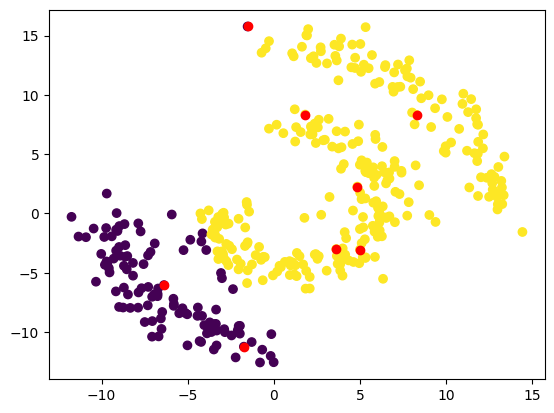
\includegraphics[width=\textwidth]{spiral_prox_r.png}
        \end{subfigure}
    \end{figure}
    \begin{center}
        \begin{tabular}{|c|c|}
            \hline
            Loss Function & Classification Accuracy (on 1 trial) \\
            \hline
            Probit & 73.0\% \\
            Regression & 63.0\% \\
            \hline
        \end{tabular}
    \end{center}
\end{frame}

\section{Conclusions}

\begin{frame}{Conclusions and Further Questions}
    \begin{itemize}

        \item Conclusions
        \begin{itemize}
            \item For well separated clusters, the method is effective, even without careful tuning

            \item Not the case for more difficult scenarios
        \end{itemize}

        \item Challenges Encountered
        \begin{itemize}
            \item Tuning of parameters - especially for real data
            \item Majority labelling
        \end{itemize}

        \item Next Steps

        \begin{itemize}
            \item Plan to apply this approach to MNIST to test on real data

            \item Anticipate tuning challenges for more difficult pairs of numbers
        \end{itemize}
        
    \end{itemize}
\end{frame}